\documentclass[a4paper,12pt]{article}
\usepackage{amssymb}
\usepackage{amsmath}
\usepackage{hhline}
\usepackage{hyperref}
\usepackage{mathtools}
\usepackage{bm}
\usepackage[margin=2cm]{geometry}

\usepackage{amsthm}


\usepackage{subcaption}

\usepackage{tabularx}
\usepackage{graphicx}
\usepackage{physics}
\usepackage{textcomp}


\graphicspath{ {./Images/} }


\newcommand{\code}[1]{\texttt{#1}}

\numberwithin{equation}{section}





\begin{document}
\title{\(1^{st}\) Challenge AN2DL}
\author{Andrea Bonifacio}
\maketitle
In this report we intend to describe the steps we made during the \(1^{\text{st}}\) challenge of the AN2DL Course. It will be covered the structure of the dataset, the first steps we made, what we did right, what we did wrong and how we decided to finally tackle the problem.
\section*{Dataset}
The dataset we were given consists in \(3452\) photos of various species of plants. Inside the main folder there are \(8\) subdirectories. In every directory there are photos of the same plant. Aside from two directories, every species has about the same number of images. The first thing we noticed is the small size of the dataset, with less then \(4000\)photos there are some limits on what we can do, Every image has a size of \(96 \times 96\) pixels, with \(3\) color channels. We opted for a 90\%/10\% split for the test and validation set.
\section*{Creating the Neural Network}
Since we were dealing with images, we opted for a Convolutional Neural Network (CNN), because we thought it was the best suited model for this kind of problem. We omitted trying a model without data augmentation because at the first run it became clear that it would only lead to overfitting, a perfect accuracy with only a \(\approx 70\%\) validation accuracy. 
\begin{figure}
      \begin{subfigure}{0.5\textwidth}

      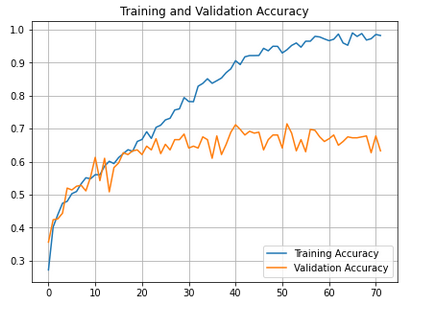
\includegraphics[scale=0.5]{model_noaug_acc.png}  
      \end{subfigure}
      \begin{subfigure}{0.4\textwidth}
            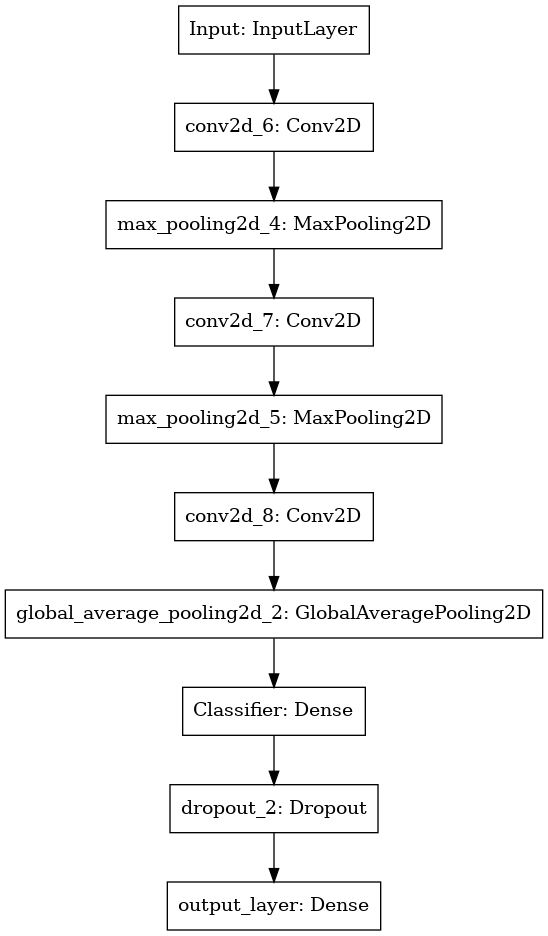
\includegraphics[scale=0.15]{model_noaug.png}
      \end{subfigure}
\end{figure}

Then, we tried to use data augmentation. Looking into Keras' documentation, we found that, inside the \code{layers} class, there were some layers specifically crafted to process images. In this way we avoided modifying the \code{model.py} file, which was a source of errors in our submissions. Using this layers we created a \code{Sequential} model which contained our image preprocessing layers. Here's an example of the model, which we added as a layer inside every model we created after:
\begin{verbatim}
    
data_augmentation = tf.keras.Sequential([
      layers.RandomCrop(80, 80),
      layers.RandomFlip("horizontal_and_vertical"),
      layers.RandomRotation((-0.2, 0.2)),
      layers.Resizing(96,96, interpolation='bicubic'),
      layers.Rescaling(1./127.5, offset=-1)])
  
\end{verbatim}
We started by adding this simple preprocessing layer to our first model and we already saw improvements to the model. Then, trying with different learning rates and batch sizes, we quickly realized that we needed to update our architecture, so we started adding layers, making two convolutions before adding a pooling layer, but what really improved our CNN was the insertion of \code{SeparableConv2D} layers. Per Keras' documentation:
\begin{quote}
      Separable convolutions consist of first performing a depthwise spatial convolution (which acts on each input channel separately) followed by a pointwise convolution which mixes the resulting output channels.
\end{quote}
It's worth noting that also many of the pretrained architectures present inside the library make extensive use of this kind of layers. Our final CNN model was able to reach an accuracy of \(\approx 81\%\) on Codalab. All the notebook with the accuracy charts will be provided alongside this report.

After this approach we decided to follow the transfer learning method, in which we pass our dataset inside a Neural Network pretrained on bigger datasets. Inside the library there are quite a few options. We decided to try two pretrained nets: Xception and VGG16. 

The idea behind transfer learning and, subsequently, fine tuning is to give the dataset to a pretrained net, which has a precise set of weights, and then unfreeze the last layers such that the net can be trained a little on the dataset. In this way it is possible to reach incredible accuracies. In our case, we tried a few different configurations, but the basic structure was always a model in which there was an input layer, followed by our data augmentation layer, then the pretrained model, a \code{Dense} layer and the output. Using Xception and fine tuning, we were able to reach an accuracy on the validation set of \(\approx 90\%\). This one was by far out best model and it performed well also on Codalab with a score of \(87\%\).w
\end{document}